% Full-wrap cover for Amazon KDP (back + spine + front).
% Compile with make_cover.py, which passes the exact dimensions:
%   \def\spinewidth{..in} \def\bleed{..in} \def\trimw{7in} \def\trimh{10in}
\documentclass{article}
\providecommand{\spinewidth}{0.90in}
\providecommand{\bleed}{0.125in}
\providecommand{\trimw}{7in}
\providecommand{\trimh}{10in}
\usepackage{calc}
\newlength{\coverw}\setlength{\coverw}{2\dimexpr\trimw\relax+\spinewidth+2\dimexpr\bleed\relax}
\newlength{\coverh}\setlength{\coverh}{\trimh+2\dimexpr\bleed\relax}
\usepackage[paperwidth=\coverw,paperheight=\coverh,margin=0pt]{geometry}
\usepackage[T1]{fontenc}
\usepackage{newpxtext}
\usepackage[scaled=0.92]{helvet}
\usepackage{xcolor}
\usepackage{tikz}
\usetikzlibrary{calc}
\definecolor{ink}{HTML}{1B2A41}
\definecolor{brand}{HTML}{0B4F6C}
\definecolor{accent}{HTML}{C8553D}
\definecolor{soft}{HTML}{EEF3F7}
\definecolor{gold}{HTML}{E9B44C}
\pagestyle{empty}
\begin{document}
\noindent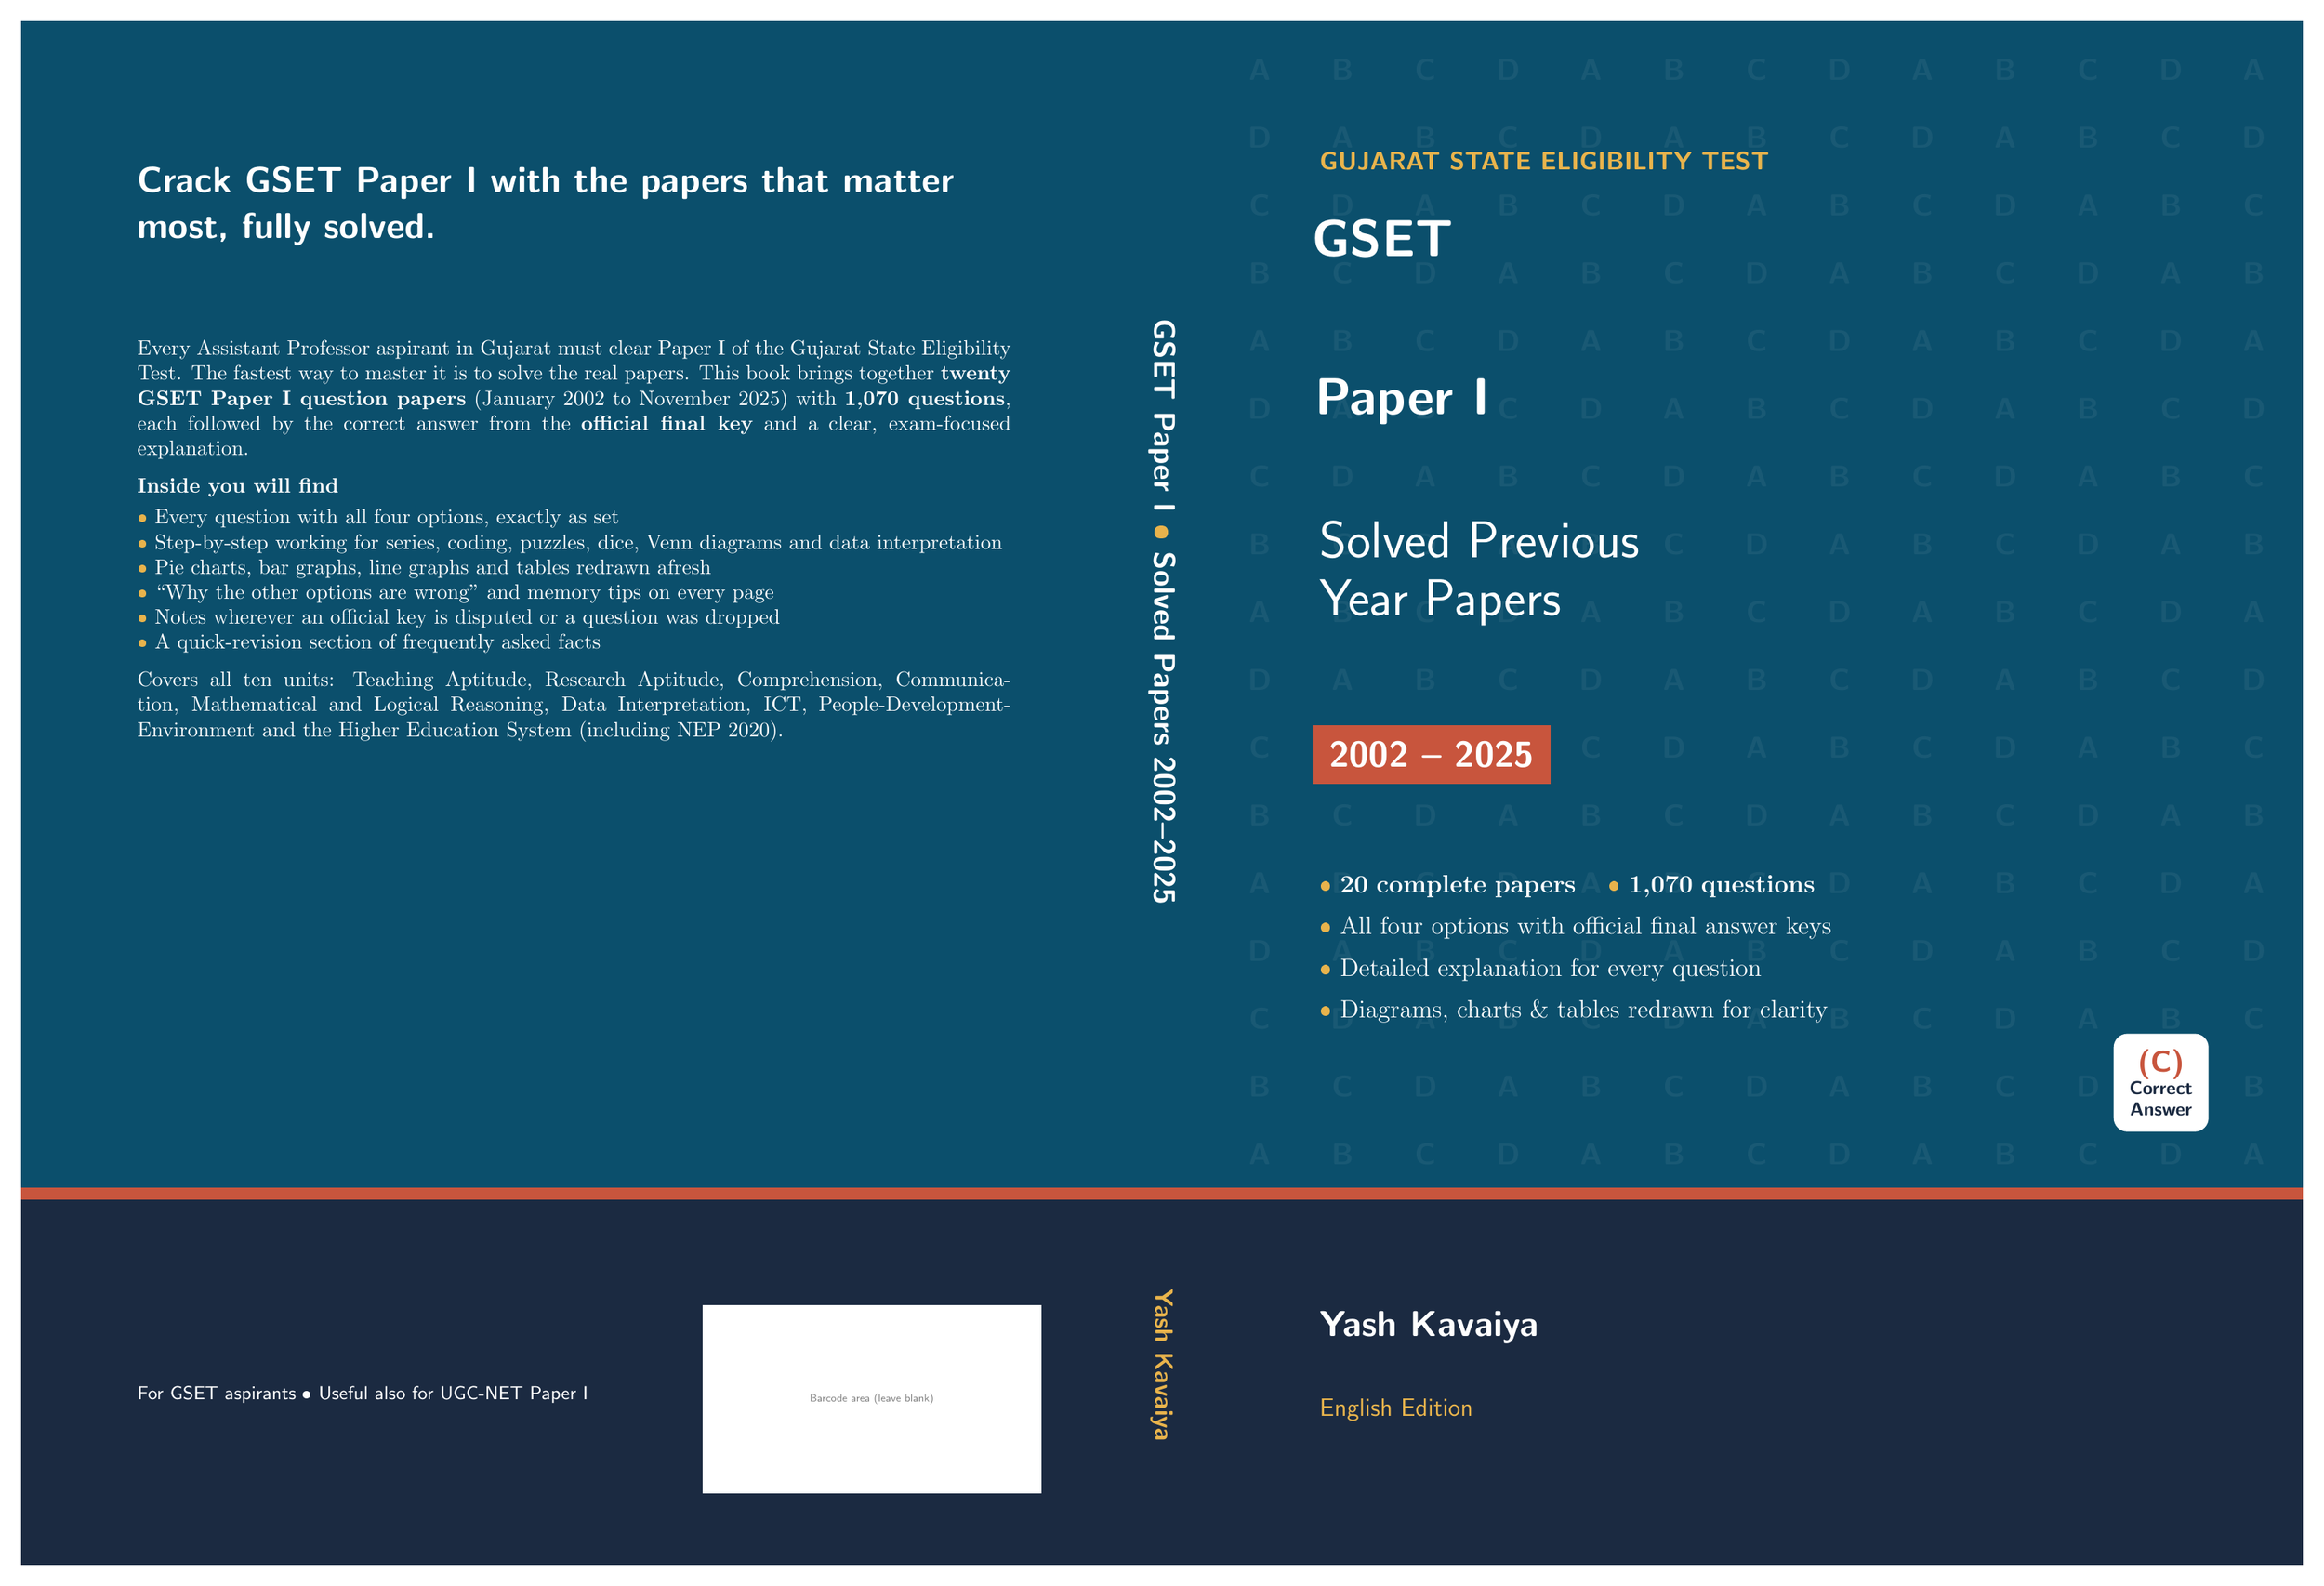
\begin{tikzpicture}[x=1in,y=1in]
% geometry (inches)
\pgfmathsetmacro{\B}{\bleed/1in}\pgfmathsetmacro{\W}{\trimw/1in}\pgfmathsetmacro{\H}{\trimh/1in}\pgfmathsetmacro{\S}{\spinewidth/1in}
\pgfmathsetmacro{\TW}{2*\W+\S+2*\B}\pgfmathsetmacro{\TH}{\H+2*\B}
\pgfmathsetmacro{\fx}{\B+\W+\S}   % left edge of front cover
\pgfmathsetmacro{\sx}{\B+\W}      % left edge of spine
% background
\fill[brand] (0,0) rectangle (\TW,\TH);
\fill[ink] (0,0) rectangle (\TW,{\B+2.3});
\fill[accent] (0,{\B+2.3}) rectangle (\TW,{\B+2.38});
% decorative grid of faint options on front
\begin{scope}
\clip (\fx,{\B+2.38}) rectangle (\TW,\TH);
\foreach \i in {0,...,14}{\foreach \j in {0,...,18}{
  \node[text=white,opacity=0.06,font=\sffamily\bfseries\Large] at ({\fx+0.2+\i*0.55},{\B+2.6+\j*0.45}) {\pgfmathparse{int(mod(\i+\j,4))}\ifcase\pgfmathresult A\or B\or C\or D\fi};}}
\end{scope}
% ---------- FRONT ----------
\node[anchor=north west,text=gold,font=\sffamily\bfseries\large,align=left] at ({\fx+0.55},{\B+\H-0.7}) {GUJARAT STATE ELIGIBILITY TEST};
\node[anchor=north west,text=white,font=\sffamily\bfseries\fontsize{58}{62}\selectfont] at ({\fx+0.5},{\B+\H-1.15}) {GSET};
\node[anchor=north west,text=white,font=\sffamily\bfseries\fontsize{40}{44}\selectfont] at ({\fx+0.52},{\B+\H-2.2}) {Paper I};
\node[anchor=north west,text=white,font=\sffamily\fontsize{24}{28}\selectfont,align=left] at ({\fx+0.55},{\B+\H-3.15}) {Solved Previous\\Year Papers};
\node[anchor=north west,fill=accent,text=white,font=\sffamily\bfseries\LARGE,inner sep=8pt] at ({\fx+0.55},{\B+\H-4.55}) {2002 -- 2025};
% feature list
\node[anchor=north west,text=white,font=\large,align=left,text width=5.6in] at ({\fx+0.55},{\B+\H-5.5}) {%
\textcolor{gold}{\textbullet}\ \textbf{20 complete papers} \quad \textcolor{gold}{\textbullet}\ \textbf{1,070 questions}\\[6pt]
\textcolor{gold}{\textbullet}\ All four options with official final answer keys\\[6pt]
\textcolor{gold}{\textbullet}\ Detailed explanation for every question\\[6pt]
\textcolor{gold}{\textbullet}\ Diagrams, charts \& tables redrawn for clarity};
% sample answer badge
\node[anchor=south east,draw=white,line width=1.2pt,rounded corners=6pt,fill=white,text=ink,font=\sffamily\bfseries,inner sep=7pt,align=center] at ({\fx+\W-0.5},{\B+2.75}) {\textcolor{accent}{\Large (C)}\\[-1pt]\small Correct\\[-2pt]\small Answer};
\node[anchor=west,text=white,font=\sffamily\bfseries\LARGE] at ({\fx+0.55},{\B+1.45}) {Yash Kavaiya};
\node[anchor=west,text=gold,font=\sffamily\large] at ({\fx+0.55},{\B+0.9}) {English Edition};
% ---------- SPINE ----------
\ifdim\spinewidth>0.4in
\node[rotate=-90,text=white,font=\sffamily\bfseries\Large] at ({\sx+\S/2},{\B+\H*0.62}) {GSET Paper I \textcolor{gold}{\textbullet} Solved Papers 2002--2025};
\node[rotate=-90,text=gold,font=\sffamily\bfseries\large] at ({\sx+\S/2},{\B+1.2}) {Yash Kavaiya};
\fi
% ---------- BACK ----------
\node[anchor=north west,text=white,font=\sffamily\bfseries\LARGE,text width=5.8in,align=left] at ({\B+0.6},{\B+\H-0.8}) {Crack GSET Paper I with the papers that matter most, fully solved.};
\node[anchor=north west,text=white,font=\normalsize,text width=5.8in,align=justify] at ({\B+0.6},{\B+\H-1.95}) {%
Every Assistant Professor aspirant in Gujarat must clear Paper~I of the Gujarat State Eligibility Test. The fastest way to master it is to solve the real papers. This book brings together \textbf{twenty GSET Paper~I question papers} (January 2002 to November 2025) with \textbf{1,070 questions}, each followed by the correct answer from the \textbf{official final key} and a clear, exam-focused explanation.\par\medskip
\textbf{Inside you will find}\par\smallskip
\textcolor{gold}{\textbullet}\ Every question with all four options, exactly as set\\
\textcolor{gold}{\textbullet}\ Step-by-step working for series, coding, puzzles, dice, Venn diagrams and data interpretation\\
\textcolor{gold}{\textbullet}\ Pie charts, bar graphs, line graphs and tables redrawn afresh\\
\textcolor{gold}{\textbullet}\ ``Why the other options are wrong'' and memory tips on every page\\
\textcolor{gold}{\textbullet}\ Notes wherever an official key is disputed or a question was dropped\\
\textcolor{gold}{\textbullet}\ A quick-revision section of frequently asked facts\par\medskip
Covers all ten units: Teaching Aptitude, Research Aptitude, Comprehension, Communication, Mathematical and Logical Reasoning, Data Interpretation, ICT, People-Development-Environment and the Higher Education System (including NEP~2020).};
% barcode area (KDP places the barcode here: keep clear)
\fill[white] ({\B+\W-2.6},{\B+0.35}) rectangle ({\B+\W-0.35},{\B+1.6});
\node[text=black!50,font=\sffamily\tiny] at ({\B+\W-1.475},{\B+0.975}) {Barcode area (leave blank)};
\node[anchor=west,text=white,font=\sffamily\small,text width=3.6in] at ({\B+0.6},{\B+1.0}) {For GSET aspirants \textbullet{} Useful also for UGC-NET Paper I};
\end{tikzpicture}
\end{document}
